\documentclass[aspectratio=169]{beamer}
\usepackage{color,amsmath}
\usepackage{subfigure}
\usepackage{booktabs}
\usepackage{framed}
\usepackage{comment}
\usepackage{ulem}

\usepackage{hyperref}
\hypersetup{
    colorlinks=true,
    linkcolor=blue,
    filecolor=magenta,      
    urlcolor=cyan,
}

%%%%%%%%%%%%%%%%%%%%%%%%%%
\title[]{\textcolor{gray}{[Introduction to mass collaboration], [Human computation],} [Open call], \textcolor{gray}{[Distributed data collection], \newline [Fragile Families Challenge]}}
\author[]{Matthew J. Salganik\\Department of Sociology\\Princeton University}
\date[]{%Summer Institutes in Computational Social Science\\2020
%\vfill
%\begin{flushleft}
%{\scriptsize
%The Summer Institutes in Computational Social Science is supported by grants from the Russell Sage Foundation and the Alfred P. Sloan Foundation.}
%\end{flushleft}
\begin{flushright}

\includegraphics[width=0.1\textwidth]{figures/cc-by.png}
\end{flushright}
}
\begin{document}
%%%%%%%%%%%%%%%%%%%%%%%%%%
\frame{\titlepage}
%%%%%%%%%%%%%%%%%%%%%%%%%%
\begin{frame}

\begin{columns}
\begin{column}{.40\textwidth}
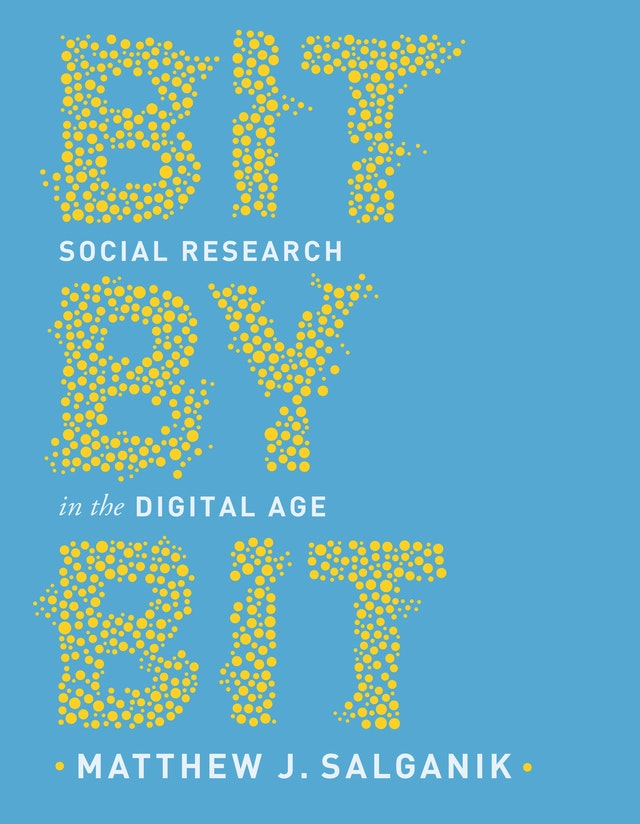
\includegraphics[width=\textwidth]{figures/salganik_bit_2018_cover}
\end{column}%

\hfill%

\begin{column}{.60\textwidth}
1) Introduction \\
2) Observing behavior \\
3) Asking questions \\
4) Running experiments \\
\textcolor{blue}{5) Mass collaboration} \\
6) Ethics \\
7) The future \\
\end{column}%
\end{columns}

\end{frame}
%%%%%%%%%%%%%%%%%%%%%%%%%
\begin{frame}

\begin{center}
\only<1>{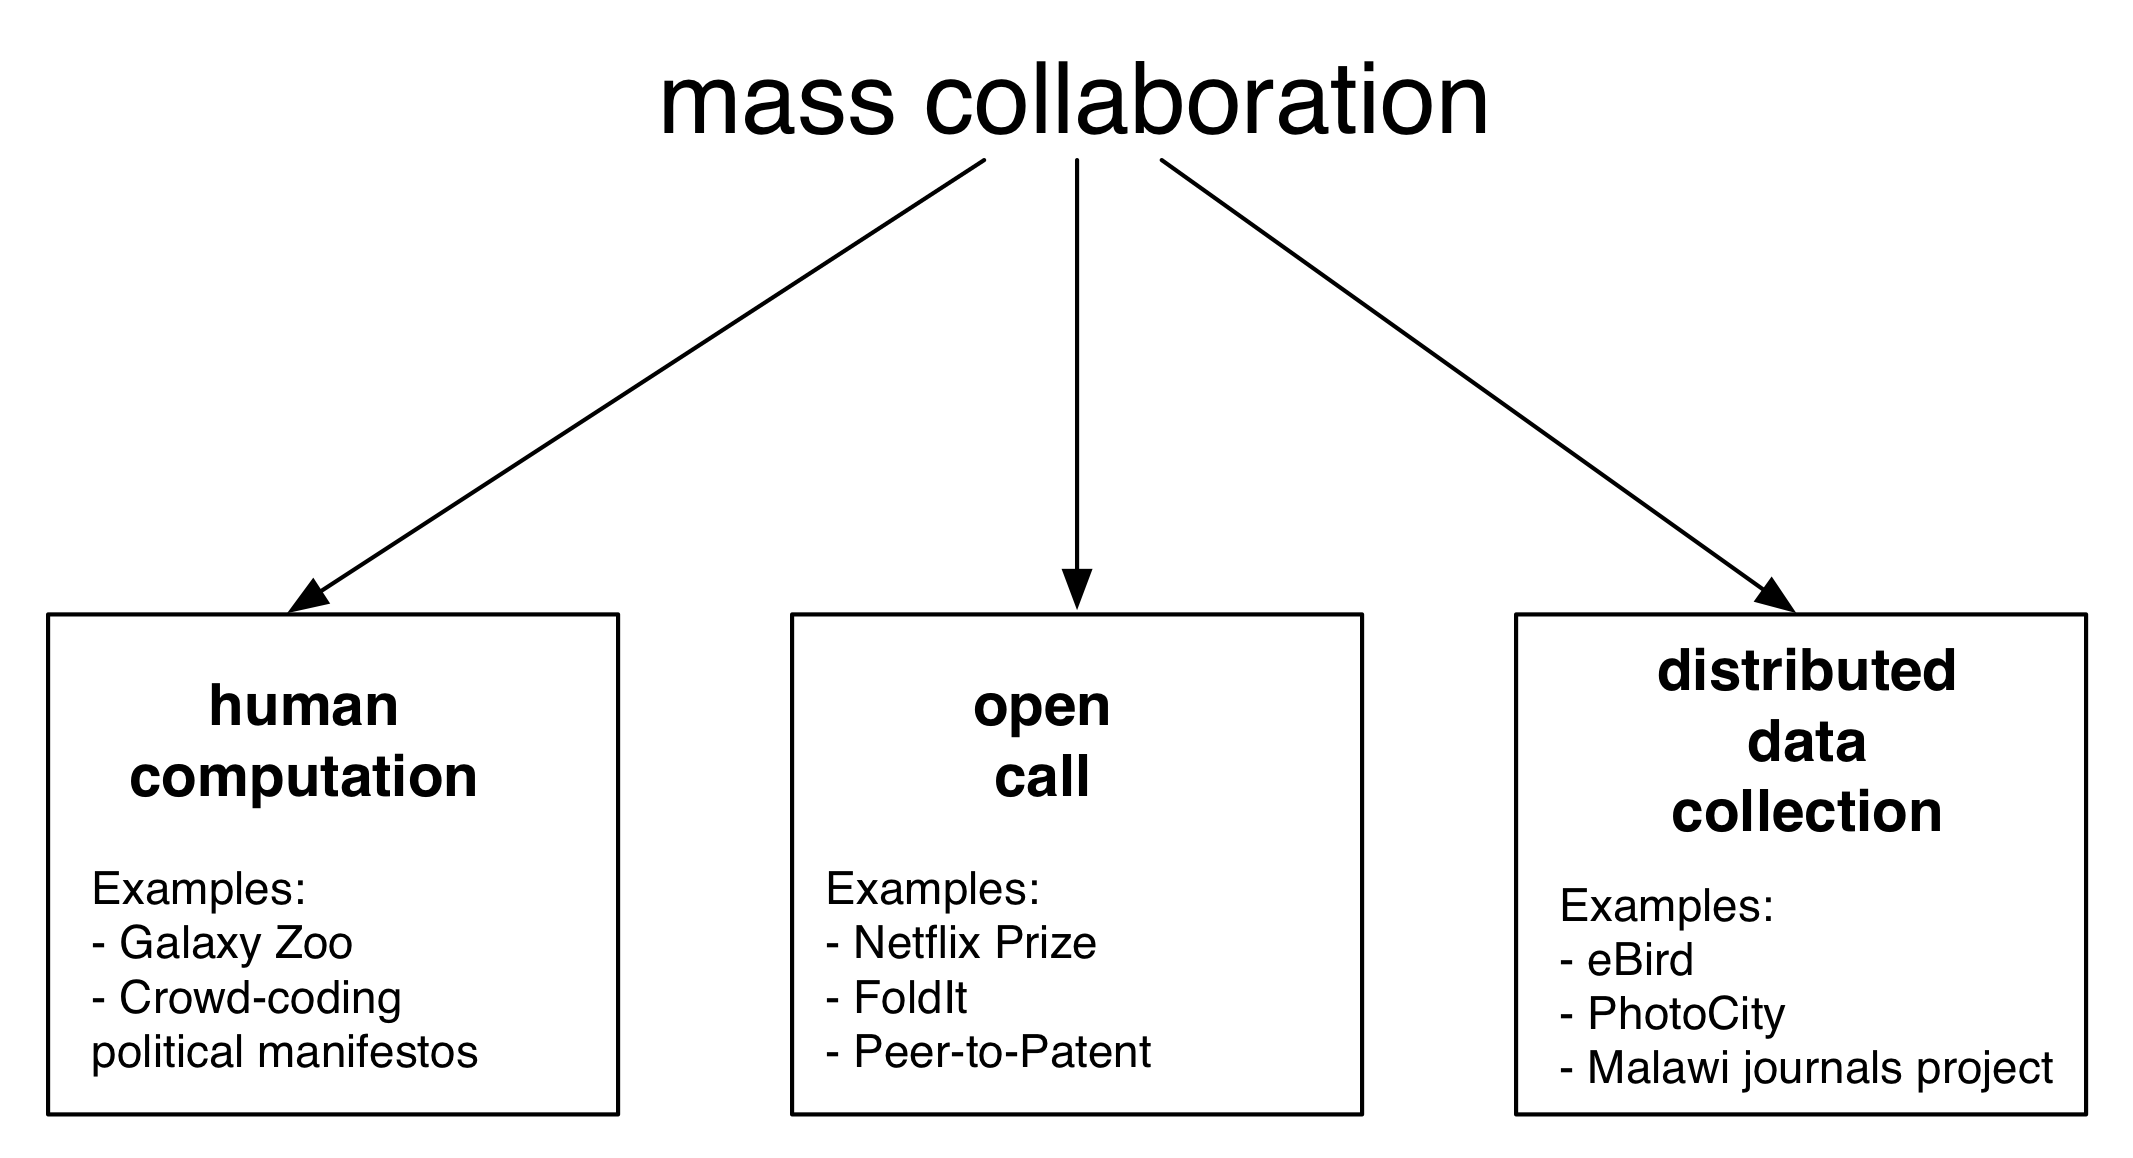
\includegraphics[width=0.9\textwidth]{figures/mass_collaboration_schematic}}
\only<2>{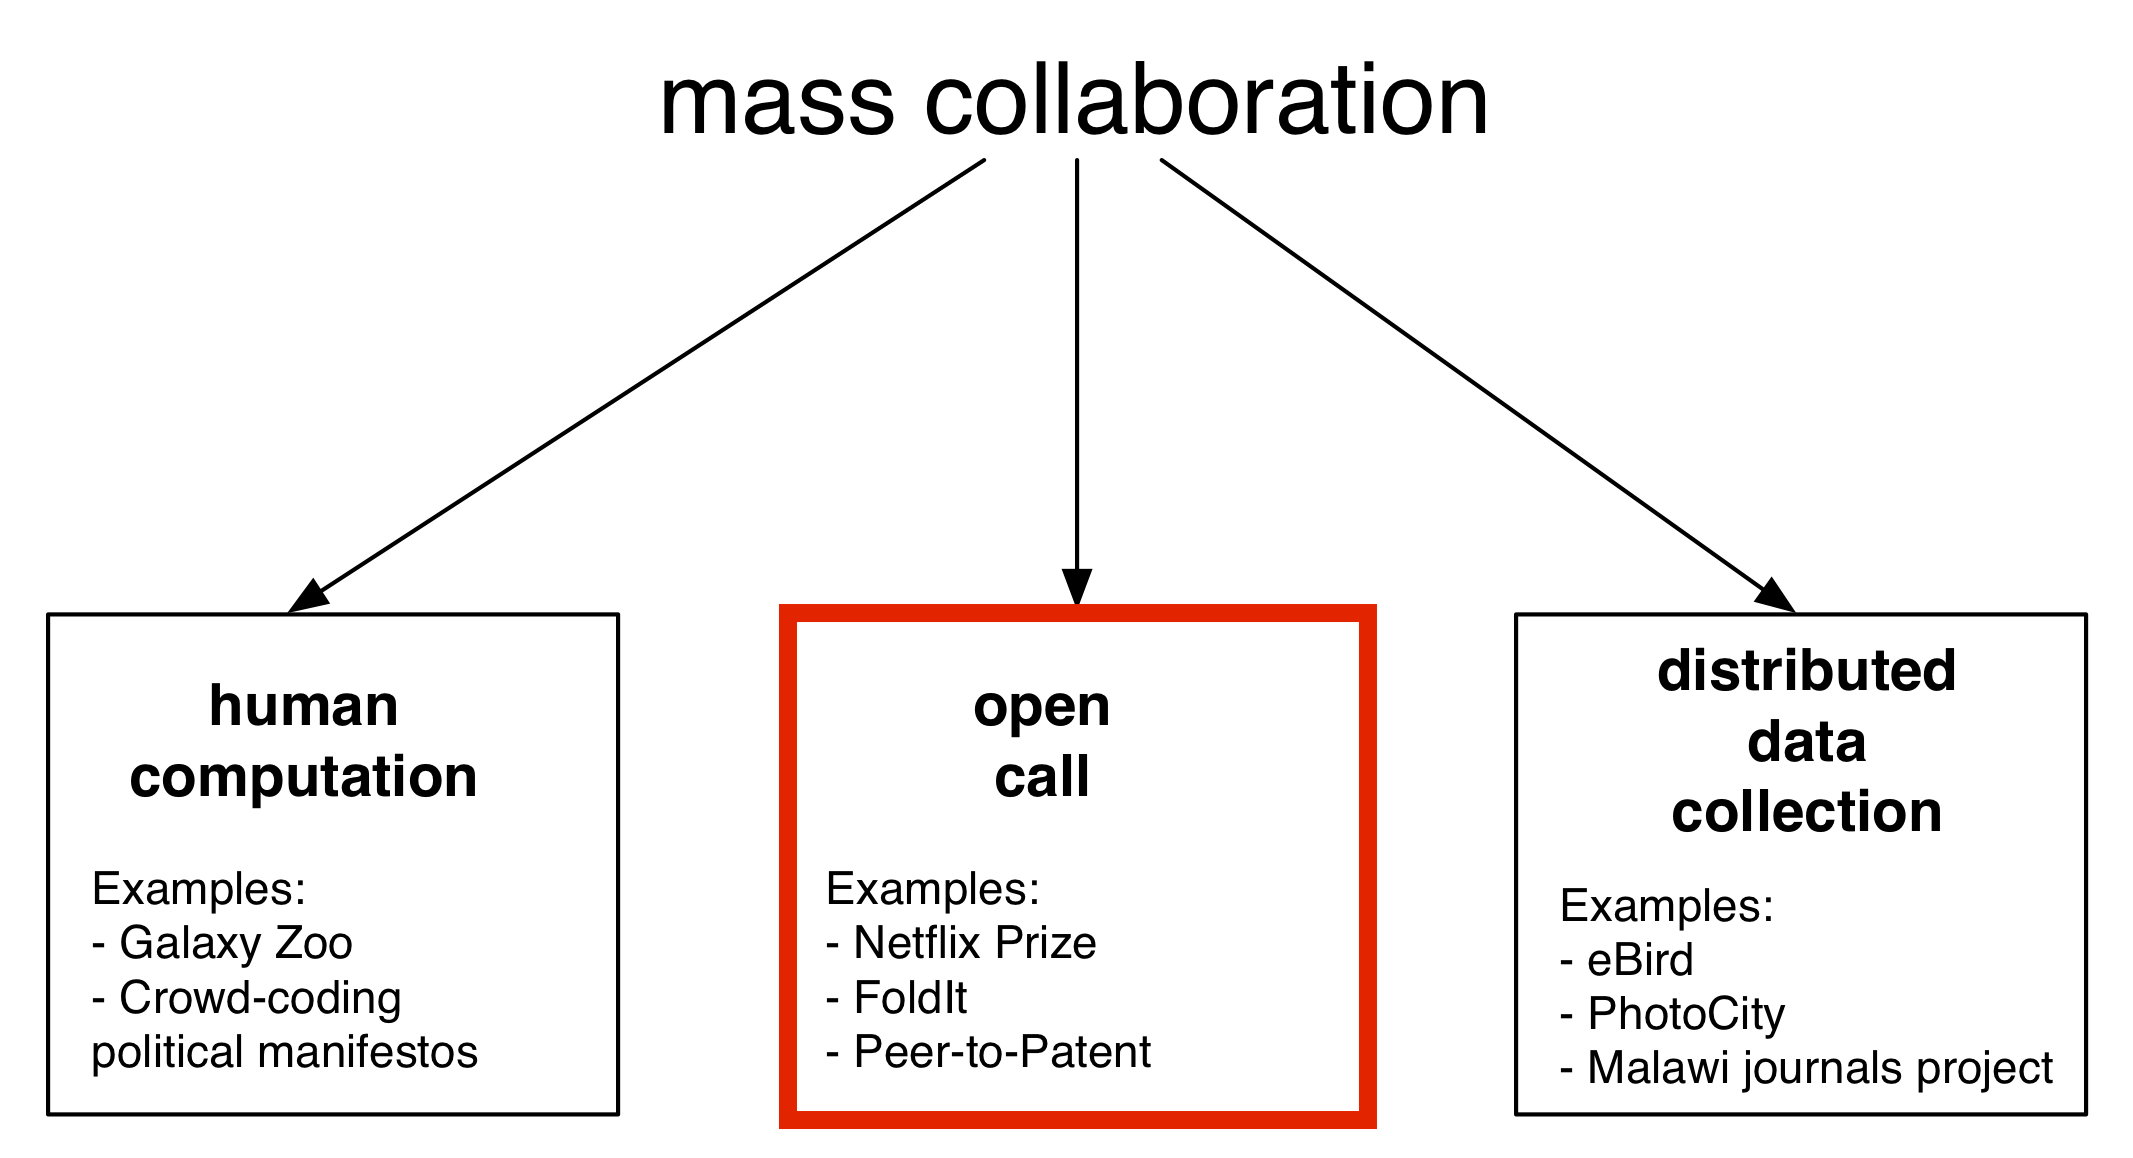
\includegraphics[width=0.9\textwidth]{figures/mass_collaboration_schematic_open_call}}
\end{center}

\vfill
Fig 5.4 (\href{https://www.bitbybitbook.com/}{Salganik 2018})
\end{frame}
%%%%%%%%%%%%%%%%%%%%%%%%%%
\begin{frame}

Open call:
\begin{itemize}
\item Problems where solutions are easier to check than generate
\pause
\item Enables easy and fair evaluation 
\pause
\item Taking the best submission (not a combination of submissions)
\pause
\item Participants require specialized skills 
\end{itemize}

\end{frame}
%%%%%%%%%%%%%%%%%%
\begin{frame}

\begin{center}
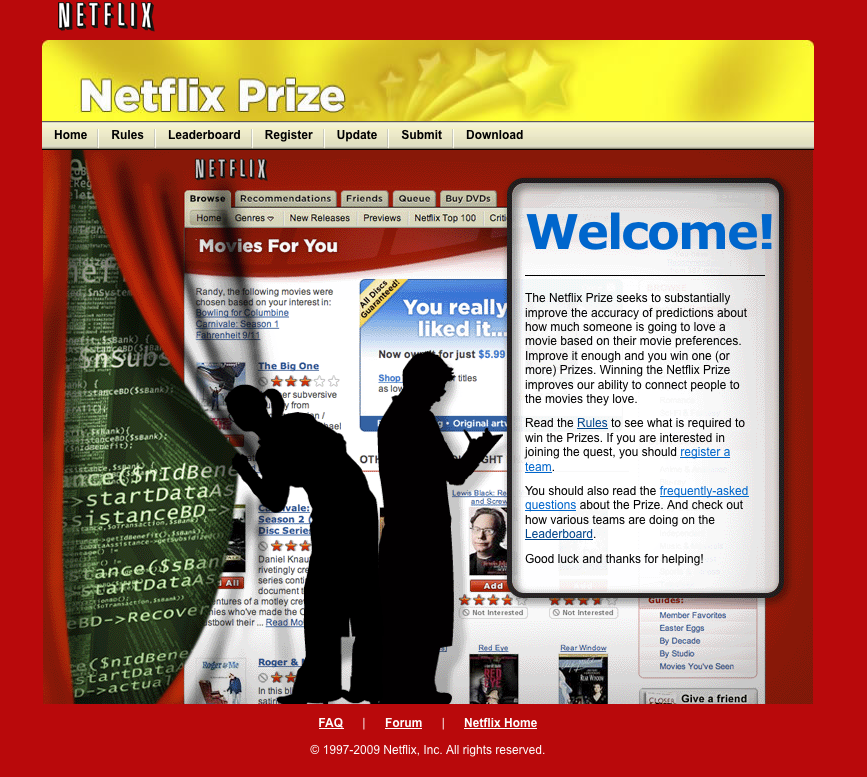
\includegraphics[height=0.8\textheight]{figures/netflix_prize}
\end{center}

\end{frame}
%%%%%%%%%%%%%%%%
\begin{frame}
\frametitle{Netflix Prize}

\begin{itemize}
\item Released a \textbf{training set} of $\sim$100 million ratings
\item Held-back a \textbf{test set} of $\sim$1.5 million ratings
\end{itemize}
\small{
\begin{tabular}{lccccccc}
           & Movie 1 & Movie 2  & Movie 3  & $\hdots$ &Movie 20,000 \\
User 1 & 2 & 5 &  & & \textcolor{blue}{?} \\
User 2 &  & \textcolor{blue}{?}  & 2  & & 3 \\
User 3 &  &  & & & 4 \\
$\vdots$ & & & & & &\\
User 500,000  & \textcolor{blue}{?} & & 2 &  & 1\\
\end{tabular}
}

\vfill
Goal is clear, but path is not clear.

\end{frame}
%%%%%%%%%%%%%%%%%
\begin{frame}
\frametitle{Netflix Prize}

\begin{itemize}
\item Open it up to the world and offer a prize of \$1,000,000
\item 44,014 valid submissions from 5,169 different teams
\item Fortunately, they were easy to check
\end{itemize}
\begin{equation*}
RMSE = \sqrt{ \frac{ \sum_i \sum_j (\widehat{r_{ij}} - r_{ij})^2}{n} }
\end{equation*}

\end{frame}
%%%%%%%%%%%%%%%%%
\begin{frame}
\frametitle{Netflix Prize}

\begin{center}
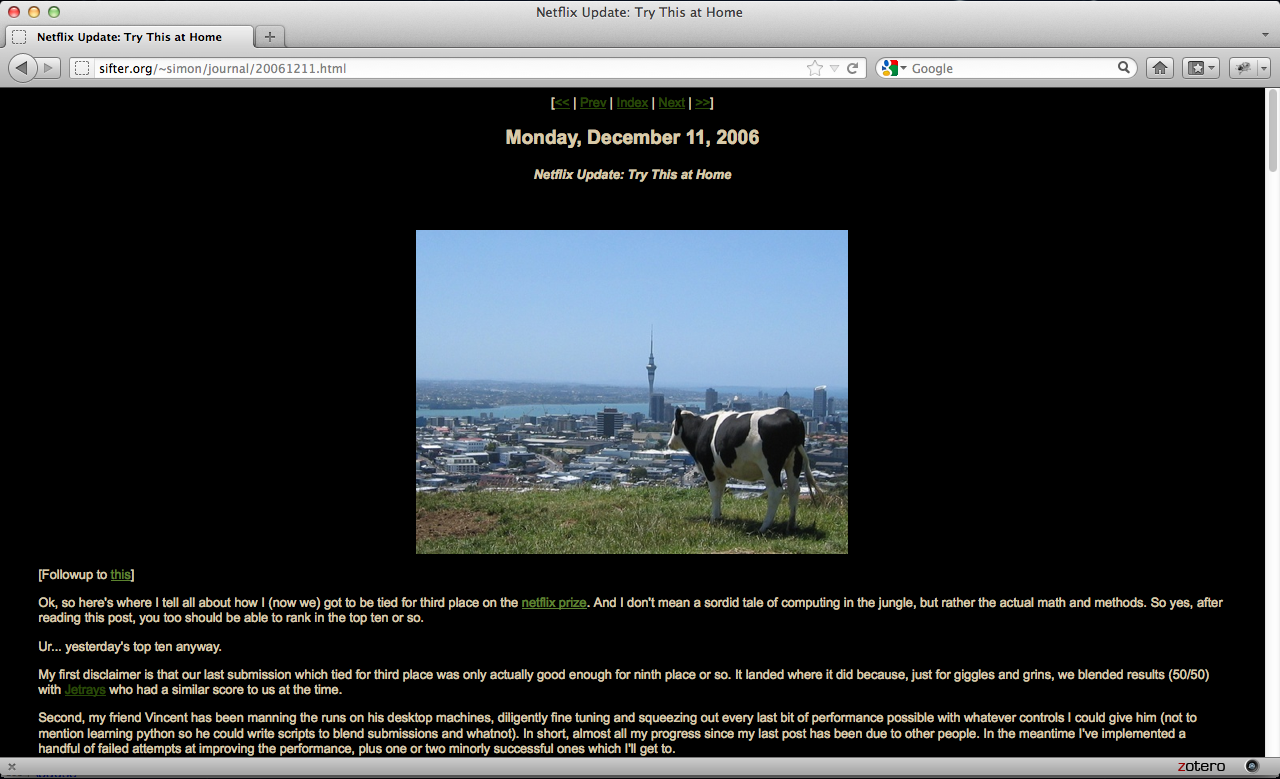
\includegraphics[width=0.95\textwidth]{figures/sifter_blog_post.png}
\end{center}

\end{frame}
%%%%%%%%%%%%%%%%%
\begin{frame}
\frametitle{Netflix Prize}

\begin{center}
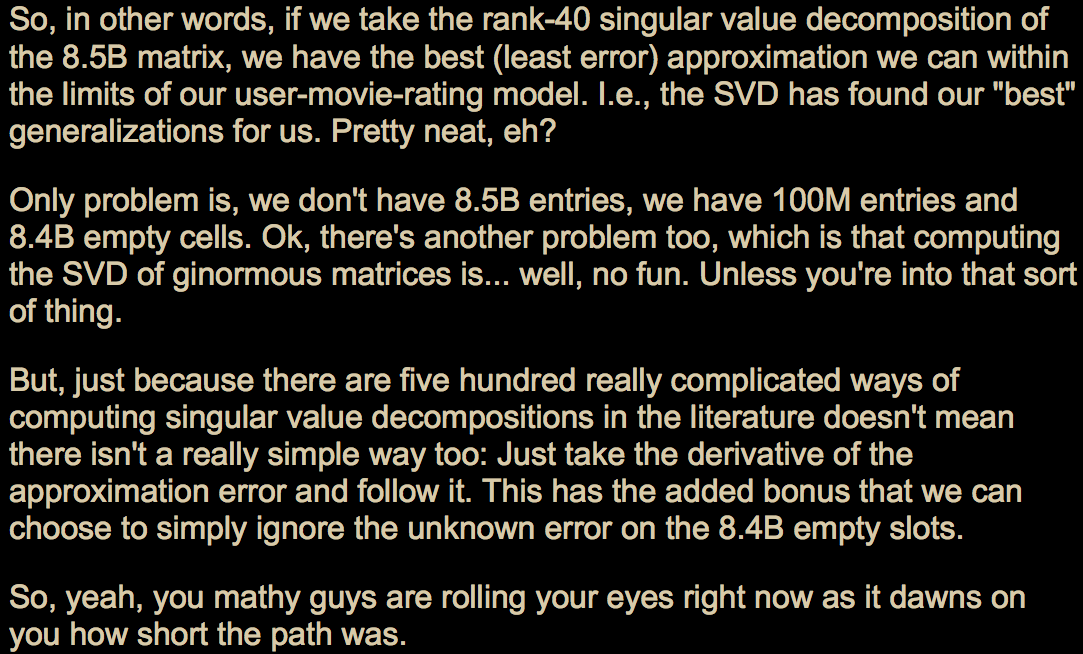
\includegraphics[width=0.7\textwidth]{figures/funk_svd_bigger}
\end{center}
\vspace{-0.2in}
Sifter aka Simon Funk
\pause
\vfill
Moved him instantly into fourth place, and was later used by all serious competitors.

\end{frame}
%%%%%%%%%%%%%%%%%%
\begin{frame}
\frametitle{Foldit}

\begin{center}
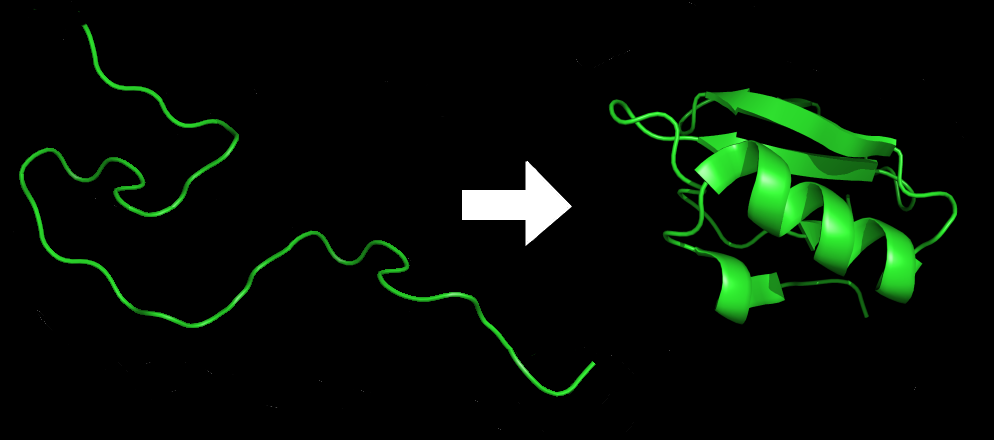
\includegraphics[width=\textwidth]{figures/bitbybit5-7_protein_folding.png}
\end{center}

\vfill
Fig 5.7 (\href{https://www.bitbybitbook.com/}{Salganik 2018})

\end{frame}
%%%%%%%%%%%%%%%%%%
\begin{frame}
\frametitle{FoldIt}

\begin{center}
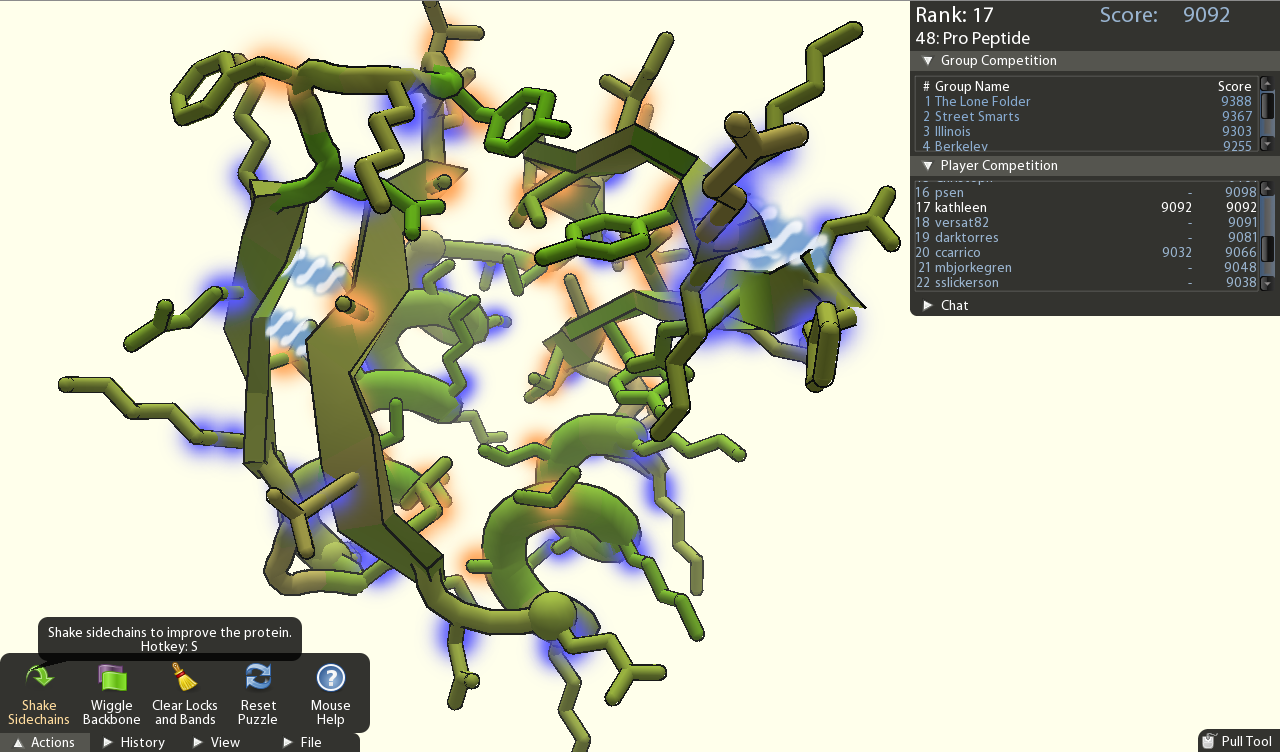
\includegraphics[width=0.8\textwidth]{figures/foldit_action}
\end{center}

\vfill
\pause
Gamers outperformed best known computational algorithms on 5 out of 10 proteins of unknown structure \href{https://rdcu.be/b4th5}{(Cooper et al., 2010)}

\end{frame}
%%%%%%%%%%%%%%%%
\begin{frame}
\frametitle{Fragile Families Challenge}

\begin{center}
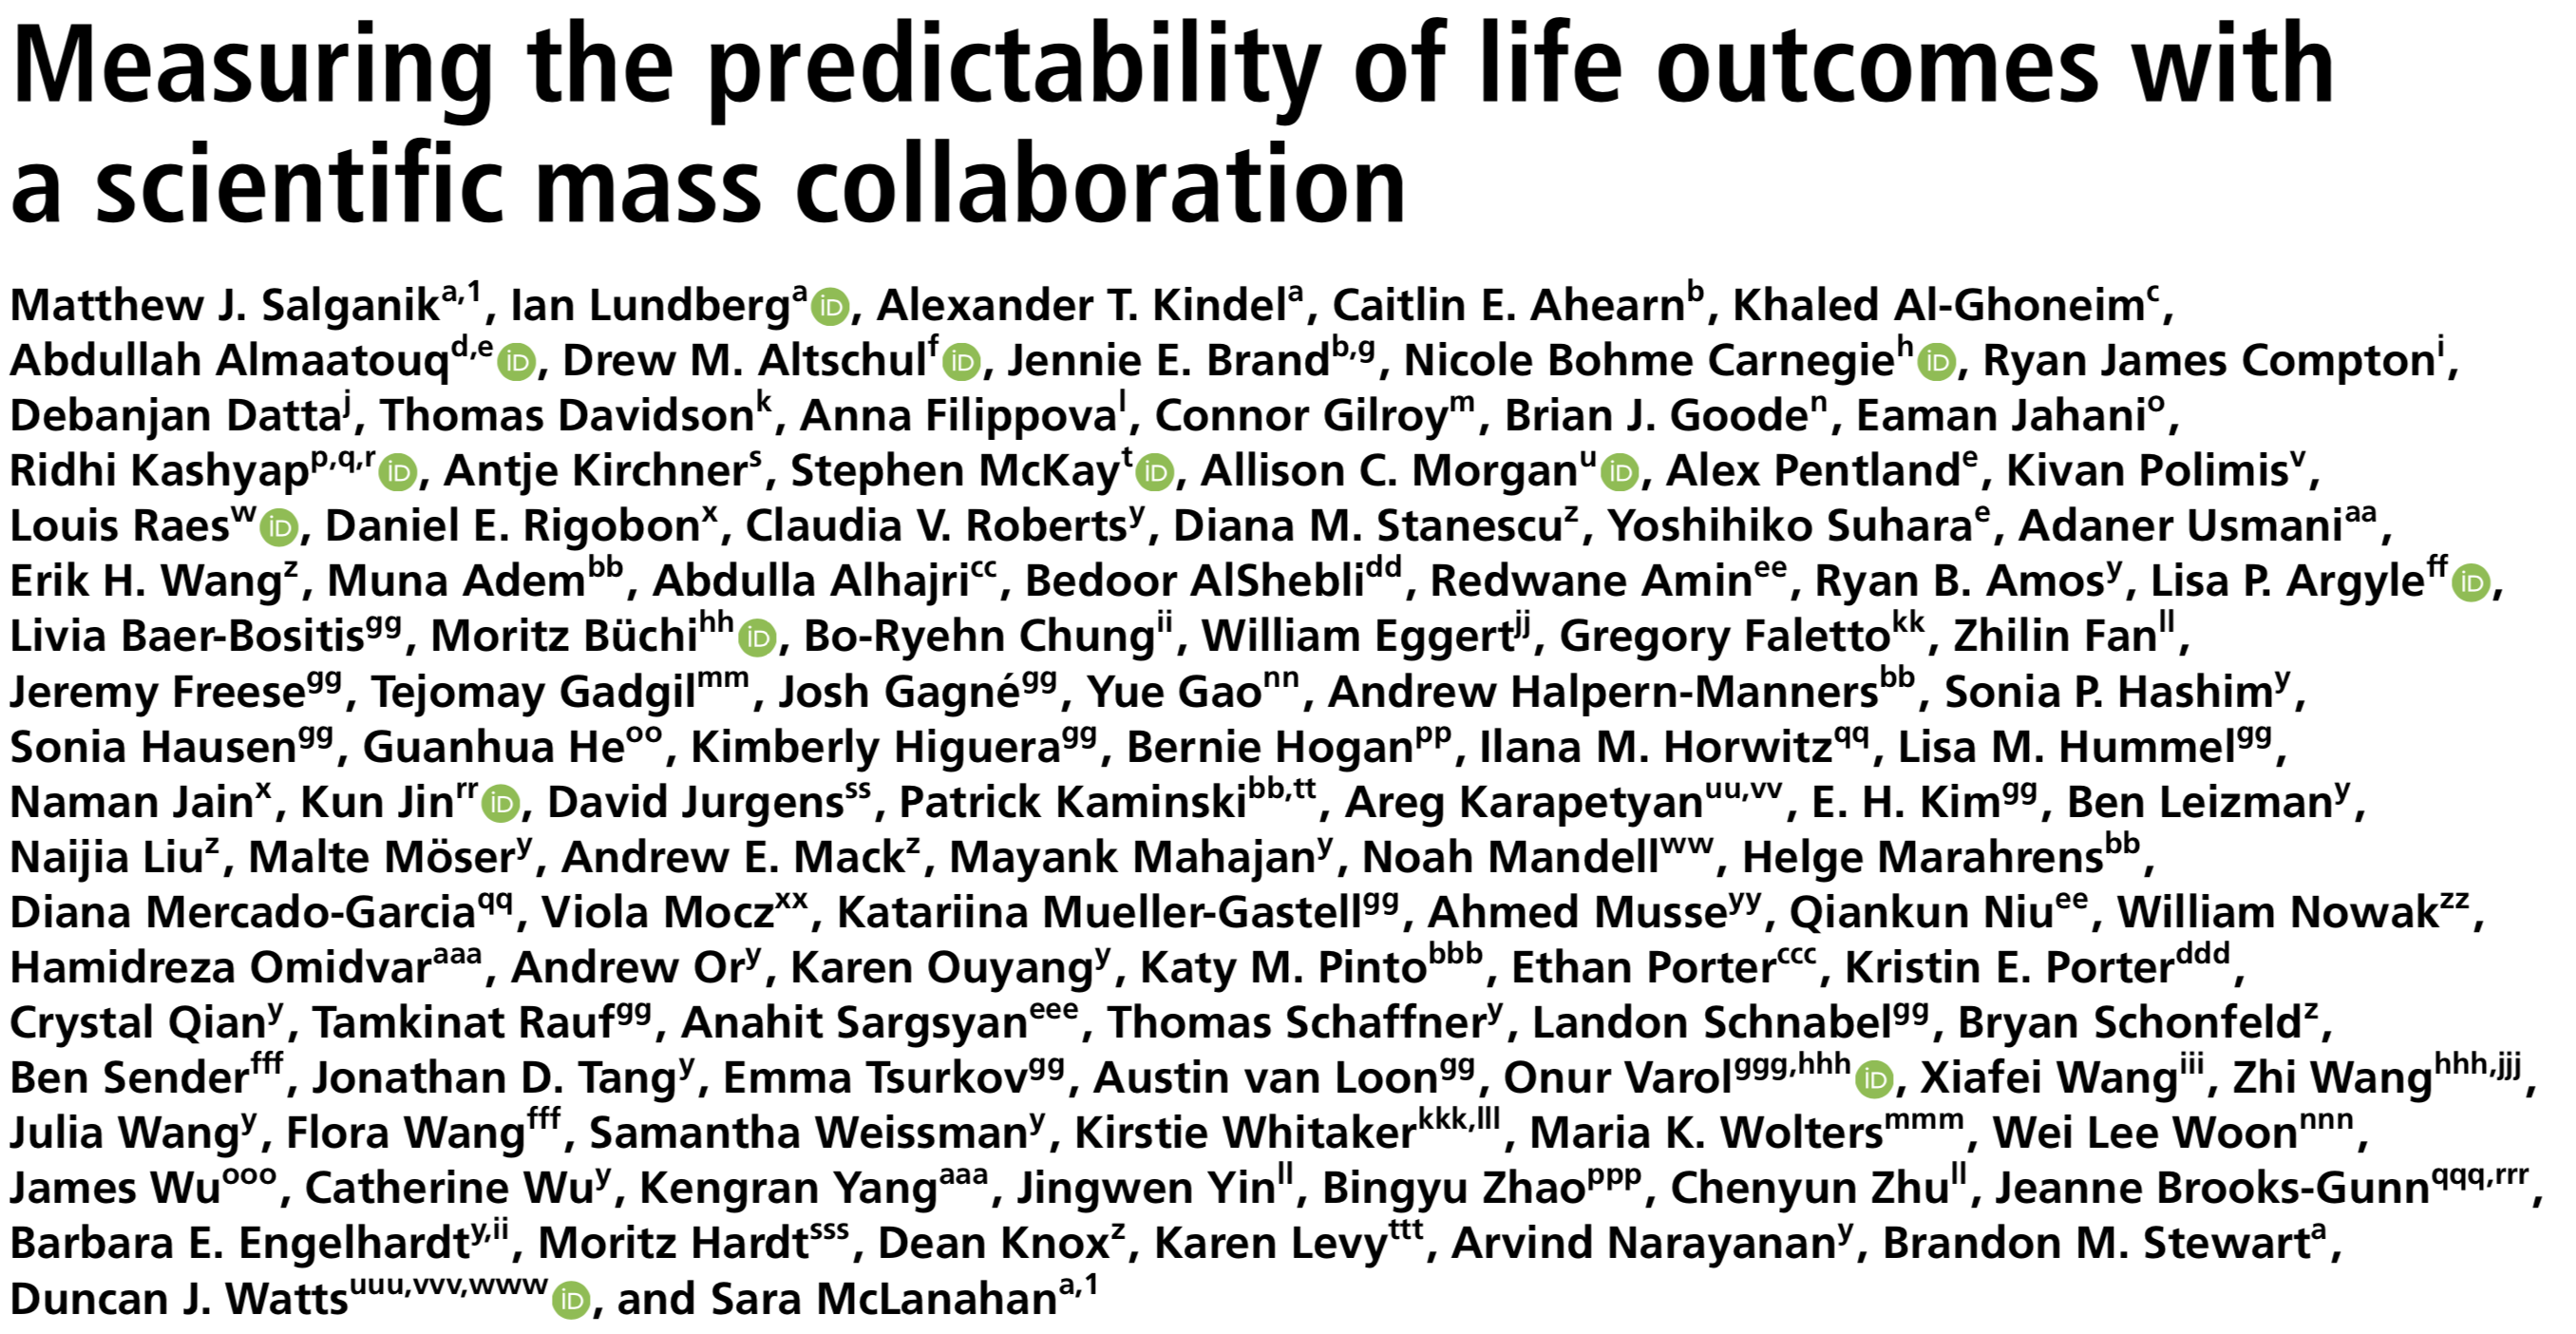
\includegraphics[width=0.8\textwidth]{figures/salganik_measuring_2020_title_authors}
\end{center}

\vfill
\href{https://doi.org/10.1073/pnas.1915006117}{(Salganik et al., 2020)}

\end{frame}
%%%%%%%%%%%%%%%%
\begin{frame}

Wrapping-up:
\begin{itemize}
\item Problems where solutions are easier to check than generate
\pause
\item Enables easy and fair evaluation 
\pause
\item Taking the best submission (not a combination of submissions)
\pause
\item Participants require specialized skills 
\end{itemize}

\end{frame}
%%%%%%%%%%%%%%%%%%%%%%%%%%
\begin{frame}

What to read next:
\begin{itemize}
\item \textit{Longitude}, Sobel (1996)
\item ``Statistical Significance of the Netflix Challenge'', \href{https://dx.doi.org/10.1214/11-STS368}{Feurverger et al.\ (2012)}
\end{itemize}

\end{frame}
%%%%%%%%%%%%%%%%%%%%%%%%
\frame{\titlepage}
%%%%%%%%%%%%%%%%%%%%%%%%%

\end{document}
